%%%%%%%%%%%%%%%%%%%%%%%%%%%%%%%%%%%%%%%%%%%%%%%%%%%%%%%%%%%%%%%%%%%%%%%%%%%%%%%
%% LaTeX-Vorlage für Abschlussarbeiten (Koma-Script)                         %%
%% (TH Köln -Campus Gummersbach, Fak. 10)                                    %%
%%                                                                           %%
%% Gemäß dem Merkblatt zur Anfertigung von Projekt-, Bachelor-, Master- und  %%
%% Diplomarbeiten der Fakultät 10 von Frau Prof. Dr. Halfmann &              %%
%% Herr Prof. Dr. Rühmann (Version vom 27.01.2008)                           %%
%%                                                                           %%
%% LIZENZ:                                                                   %%
%% Diese Vorlage darf nicht kommerziell verbreitet                           %%
%% werden. Eine nicht-kommerzielle Weitergabe ist                            %%
%% gestattet.                                                                %%
%%                                                                           %%
%% Von Ludger Schönfeld, M. Sc.,                                             %%
%% 2015-2017 (Stand: 05.04.17)                                               %%
%%%%%%%%%%%%%%%%%%%%%%%%%%%%%%%%%%%%%%%%%%%%%%%%%%%%%%%%%%%%%%%%%%%%%%%%%%%%%%%

\documentclass[a4paper,fontsize=12pt,abstract=true, toc=nolistof,headsepline=true,footsepline=true]{scrartcl}
%%INFO: Dokumenteinstellungen
% - fontsize: Schriftgröße (hier jede beliebige, Standard: 11pt)
% - abstract: Überschrift zum Abstract ein-/abschalten (Werte: true/false)
% - toc: Gestalt des Inhaltsverzeichnisses beeinflussen (s. KOMA-Script-Guide).
%   Wert "listof/nolistof" => Verzeichnisse von Tabellen & Abbildungen werden unnummeriert ins Inhaltsverzeichnis aufgenommen bzw. nicht ins Inhaltsverzeichnis aufgenommen.
% - headsepline: Ein-/Ausschalten einer Linie in der Kopfzeile.
% - footsepline: Ein-/Ausschalten einer Linie in der Fusszeile.
%

\usepackage[ngerman]{babel}
\usepackage[T1]{fontenc} % Schriftkodierung (Für Sonderzeichen u.a.)
\usepackage[utf8]{inputenc} % Für die direkte Eingabe von Umlauten im Editor u.a. - ACHTUNG: Kodierung muss mit der Zeichenkodierung im Editor übereinstimmen!
\usepackage{microtype} % Verbesserter Randausgleich
\usepackage{lmodern}
\usepackage{parskip}

%% Paket für Beispiel-Text (Pseudo-Latein)
% => Befehl (Bsp.): \lipsum[2-4]
\usepackage{lipsum}

%% Zeilenabstand setzen
\usepackage[onehalfspacing]{setspace}
% INFO: Zeilenabstand setzen:
%
% Befehle:
% - \singlespacing  => 1-zeilig (Standard)
% - \onehalfspacing => 1,5-zeilig
% - \doublespacing  => 2-zeilig

%% Satzspiegel einrichten
\usepackage[left=3cm,right=2cm,top=1.5cm,bottom=1cm,
    textheight=245mm,textwidth=160mm,includeheadfoot,headsep=1cm,
    footskip=1cm,headheight=14.599pt]{geometry} % Einrichtung der Seite
% KOMA-Script bietet das Paket "typearea". Dieses berechnet Ihnen eine optimale Seiteneinstellung. Bei diesem Paket haben Sie allerdings nicht so viele Einstellungsmöglichkeiten.

%% Einstellungen für Marginalien (Beispiel)
%%(Randkommentierung mit \marginpar{Text})
%\newcommand\mpar[1]{\marginpar {\flushleft\sffamily\small #1}}
%\setlength{\marginparwidth}{3cm}

%% Einbinden von Graphiken
\usepackage{graphicx}
\usepackage{epstopdf} % Umwandlung EPS-Bilder => PDF, sodass diese auch mithilfe des Tools "pdflatex" eingebunden werden können
% Unterstreichen von Text
\usepackage[normalem]{ulem} % Befehl: \uline{}

%% Pakete für Tabellen
\usepackage{tabularx} % Einfache Tabellen
\usepackage{longtable} % Tabellen als Gleitobjekte (für die Aufteilung bei langen Tabellen über mehrere Seiten)
\usepackage{multirow} % Verbinden von Zeilen innerhalb einer Tabelle mit \multirow{anzahl}{*}{Text}
\usepackage{pbox}

% (Zusatz-)Pakete für Formeln
\usepackage{amsmath}
\usepackage{amsthm}
\usepackage{amsfonts}

% Farbboxen (für die Merkkästen in dieser Vorlage):
\usepackage{tcolorbox}
\tcbset{colback=white,colframe=orange,
    fonttitle=\bfseries}

%% Autom. Literaturverzeichnisse mit dem Paket 'biblatex'":
\usepackage{biblatex}
\addbibresource{bib/sources.bib}

\usepackage[colorlinks,pdfpagelabels,pdfstartview=FitH,
    bookmarksopen=true,bookmarksnumbered=true,linkcolor=black,
    plainpages=false,hypertexnames=false,citecolor=black]{hyperref} % Für Verlinkungen
% INFO: Verlinkungen mit dem hyperref-Paket:
%
% Die Angabe von URLs mit dem Befehl \url{} erlaubt einen
% gesonderten Umgang mit Weblinks. Denn die Links werden verlinkt.
% Auch erfolgt automatisch am Zeilenende ein Umbruch des Links.
% Es ist auch nicht erforderlich, Sonderzeichen in der URL manuell zu
% entschärfen.
%
% TIPP: Sollte ein Umbruch bei einem Link nicht automatisch erfolgen, so kann
% das daran liegen, dass ein/mehrere Zeichen zusätzlich angegeben werden müssen,
% an dem der Link umbrochen werden kann.
% => Siehe Paket "breakurl"

\usepackage{pdfpages}

\usepackage{color}
\usepackage{xcolor}

\usepackage{array,etoolbox}
\usepackage{csquotes}
\preto\tabular{\setcounter{magicrownumbers}{0}}
\newcounter{magicrownumbers}
\newcommand\rownumber{\stepcounter{magicrownumbers}\arabic{magicrownumbers}}

\newcommand{\newlineparagraph}[1]{\paragraph{#1}\mbox{}\\}

\begin{document}
    \pagestyle{empty}
\begin{titlepage}
    
\includegraphics[scale=1.0]{assets/logo_TH-Koeln_CMYK_22pt}\\
    \begin{center}
        \large
        Technische Hochschule Köln\\
        Fakultät für Informatik und Ingenieurwissenschaften\\
        \vspace{1cm}
        \large
        \textsc{Bachelorarbeit}\\
        \vspace{1cm}
        \huge
        Vergleichende Analyse von\\
        Laravel Admin-Panels mittels\\
        Software Design Principles und Patterns\\
        sowie prototypischer Implementierung\\
        \vspace{1cm}
        \large
        vorgelegt an der TH Köln\\
        Campus Gummersbach\\
        im Studiengang\\
        Medieninformatik\\
        \vspace{1cm}
        ausgearbeitet von:\\
        \textsc{Niklas Canisius}\\
        (Matrikelnummer: 11110023)\\
        \vspace{1cm}
        \begin{tabular}{ll}
            \textbf{Erster Prüfer:} & Prof.\ Dr. Christian Kohls \\
            \textbf{Zweiter Prüfer:} & Johannes Frielingsdorf \\
        \end{tabular}
        \vspace{1cm}
        \\Gummersbach, den \today
    \end{center}
\end{titlepage}

    \newpage


\section*{Sperrvermerk}
Das vorliegende Dokument beinhaltet vertrauliche Daten der Firma Graw Radiosondes GmbH \& Co. KG.
Es darf nur von berechtigten Personen innerhalb ihrer dienstlichen Verpflichtungen eingesehen werden.

Eine Veröffentlichung und Vervielfältigung – auch in Teilen – ist nicht gestattet.
Dritten darf dieses Dokument nur mit der ausdrücklichen Genehmigung des Verfassers und des Unternehmens zugänglich gemacht werden.

Der Sperrvermerk gilt für ein Jahr ab dem \today.

    %\newpage


\section*{Abstract}


    \newpage
    \renewcommand{\contentsname}{Inhaltsverzeichnis}
    \tableofcontents
    \newpage

    \pagestyle{headings} % Kopf- und Fußzeilen aktivieren
    \pagenumbering{arabic} % Seitennummerierung: arabische Zahlen

    \section{Einleitung}

Diese Arbeit baut auf der vorangegangenen Praxisprojektarbeit auf.
Diese trägt den Titel \enquote{Praktische Evaluation des Frameworks Laravel Nova am Beispiel einer Anwendung zur Verwaltung und Auswertung von Radiosondenaufstiegen}.
In dieser Arbeit zeigten sich Probleme mit Nova, vor allem in puncto Anpassbarkeit.
Ebenfalls wurden in einer Nutzwertanalyse geeignete Alternativen zu Nova identifiziert.
Dabei wurde vor allem das Framework filament~\cite{filament} als bessere Alternative herausgearbeitet.
Unter Betrachtung dieser kurzen Vorstudie entsteht die Bachelorarbeit.
Die beiden Frameworks Nova und filament sollen anhand von Software Design Principles und Patterns, sowie prototypischer Implementierung, verglichen werden.

\subsection{Fragestellung}
Im Rahmen dieser Arbeit soll die Frage geklärt werden, ob für das vorliegende Projekt der \enquote{Sounding Console} Nova oder filament besser geeignet ist.

\subsection{Zielsetzung}
Ziel dieser Arbeit ist zum einen die prototypische Umsetzung einiger Features der Sounding Console mittels filament.
Dabei sollen praktische Erfahrungen mit dem Framework gesammelt werden um diese mit den bei Nova vorhandenen Erfahrungen zu vergleichen.

Zum anderen soll ein theoretischer Vergleich der beiden Frameworks durchgeführt werden.

Als finales Ergebnis soll die Fragestellung bewertet werden und damit der weitere Weg für die Applikation bestimmt werden.

    \section{Grundlagen}
Die theoretische Basis für den Vergleich bieten verschiedene Software Design Principles und Patterns, welche
im Folgenden eingeführt werden.

\subsection{Principles}
Software Design Principles sind weder Regeln, Gesetze noch perfekte Wahrheiten.
Stattdessen sind diese Prinzipien Empfehlungen bzw.\ Ratschläge.
(Vgl.~\cite{getting-a-solid-start})

Software Design Prinzipien sind Heuristiken und allgemeingültige Lösungen für übliche Probleme.
Sie wurden empirisch beobachtet und gelten daher meistens, allerdings auch nicht unbedingt immer.
(Vgl.~\cite{getting-a-solid-start})

https://www.geeksforgeeks.org/principles-of-software-design/

https://www.dotnettricks.com/learn/designpatterns/different-types-of-software-design-principles

\subsubsection{SOLID Principles}
Die Kerngruppe der Software Design Prinzipien werden von Robert C. Martin unter dem Titel \enquote{The Principles of OOD}(\cite{solid}) beschrieben.
Die Grundlage dafür legte er in seinem Paper \enquote{Design Principles and Design Patterns}(\cite{design-principles-and-design-patterns}) im Jahr 2000.

https://medium.com/successivetech/s-o-l-i-d-the-first-5-principles-of-object-oriented-design-with-php-b6d2742c90d7

https://www.digitalocean.com/community/conceptual-articles/s-o-l-i-d-the-first-five-principles-of-object-oriented-design#interface-segregation-principle

https://accesto.com/blog/solid-php-solid-principles-in-php/

\paragraph{Single Responsibility Principle}
\enquote{A class should have one, and only one, reason to change.}(\cite{solid})

\paragraph{Open Closed Principle}
\enquote{You should be able to extend a classes' behavior, without modifying it.}(\cite{solid})

\paragraph{Liskov Substitution Principle}
\enquote{Derived classes must be substitutable for their base classes.}(\cite{solid})

\paragraph{Interface Segregation Principle}
\enquote{Make fine-grained interfaces that are client specific.}(\cite{solid})

\paragraph{Dependency Inversion Principle}
\enquote{Depend on abstractions, not on concretions.}(\cite{solid})

\subsubsection{Boy Scout Rule}
Sinnvoll im Projektkontext?
\subsubsection{PSR (PHP Standards Recommendations)}
The PHP Framework Interop Group is working on and publishes PSRs (PHP Standards Recommendations).(Vgl. \cite{psr})

\subsubsection{KISS (Keep It Simple Stupid)}
\begin{itemize}
    \item Don't complicate the code.
    \item The code should be its documentation itself.
    \item Any new programmer on the team should be able to get into the project quickly.
\end{itemize}
\subsubsection{DRY (Don’t Repeat Yourself)}
Do not code using the Copy-Paste principle (there is no such rule).

See that the same code repeats in several places? Extract code for a separate function.
\subsubsection{YAGNI (You Aren’t Gonna Need It)}
We should not write code “for the future”.

Such code is not needed at the moment.
\subsubsection{GRASP (General Responsibility Assignment Software Patterns)}
GRASP is a large set of rules about which I could write a separate article.
These are the basic principles that we should follow when creating object design and responsibility assignments.
It consists of: Information Expert, Controller, Creator, High Cohesion, Low Coupling, Pure Fabrication, Polymorphism, Protected Variations, Indirection.

\subsection{Patterns}
Patterns, sogenannte Entwurfsmuster, wurden ursprünglich vom Architekten Christopher Alexander geprägt.
Dieser beschrieb in seinem Buch \enquote{A Pattern Language: Towns, Buildings, Construction}(\cite{a-pattern-language}) im Jahr 1977 zum ersten Mal Muster, unter dessen Einsatz man immer wiederkehrende Probleme lösen kann.
In der Informatik wurden Entwurfsmuster durch die Veröffentlichung der \enquote{Gang of Four} im Jahr 1994 populärer.
In ihrem Buch \enquote{Design Patterns - Elements of Reusable Object-Oriented Software}(\cite{gamma-design-patterns}) beschreiben Erich Gamma et al.\ 23 unterschiedliche Entwurfsmuster.
Diese sind eingeteilt in die drei Kategorien Creational, Structural und Behavioral.

1999 ergänzte Martin Fowler in \enquote{Patterns of Enterprise Application Architecture}(\cite{patterns-of-enterprise-application-architecture}) die Kategorie \enquote{Objektrelationale Abbildung} und dazugehörige Muster.
Gregor Hohpe und Bobby Woolf ergänzten 2003 die Kategorie der Messaging Patterns in ihrem Buch \enquote{Enterprise Integration Patterns}(\cite{enterprise-integration-patterns}).

Die Menge der Entwurfsmuster ist so umfangreich, dass eine wiedergabe aller an dieser Stelle weder von Nutzen noch machbar wäre.
Im Folgenden werden daher nur die Muster eingeführt, die im anschließenden Vergleich verwendet werden.

    \newpage


\section{Analyse}
Die Basis für den theoretischen Teil liefern die skizzierten Software Design Principles und Patterns.
Im Rahmen der weiteren Analyse wird geklärt, welche Principles und Patterns im vorliegenden technischen Anwendungskontext grundsätzlich zur Anwendung kommen können.

Grundlage für den praktischen Teil dieser Arbeit ist die auf Basis von Laravel und Nova entwickelte Sounding Console.
Um den Funktionsrahmen für den weiteren Prototypen zu definieren, sind zunächst die Probleme mit dem bestehenden MVP (Minimal Viable Product) zu identifizieren.

Weiterhin bietet der jeweilige Funktionsumfang der Frameworks eine sinnvolle Vergleichsbasis.
Dafür wird eine geeignete Vergleichsmethodik identifiziert, definiert und durchgeführt.

Weitere mögliche Vergleichsaspekte sind die Maturity der beiden Frameworks, der verwendete Code Style, ein Kostenvergleich und Unterschiede in der Lizenzierung.
Inwiefern diese Aspekte vergleichbar sind, ist ebenfalls Gegenstand dieser Analyse.

\subsection{Geeignete Principles und Patterns}
Die Auswahl der Principles und Patterns im Grundlagenteil dieser Arbeit wurde bereits dargestellt:
Nicht jedes Pattern passt in jeden Kontext.
Im Folgenden wird begründet, warum die skizzierten Principles und Patterns im vorliegenden Projektkontext überprüft werden.

\subsubsection{Geeignete Principles}
Die Sounding Console folgt dem Konzept der objektorientierten Entwicklung.
Dafür sind die SOLID Principles entworfen und für das vorliegende Projekt anwendbar.

Die Prinzipien KISS, DRY und YAGNI sind generell für unterschiedlichste Softwareprojekte konzipiert.
Daher wird der Einsatz der Frameworks untersucht auf Einfachheit, Wiederholungen und vorbereitenden, jedoch nicht notwendigen Code.

Filament und Nova sind, abgesehen vom Frontend, in PHP geschrieben.
Beim Einsatz der Frameworks wird fast ausschließlich PHP verwendet.
Die PSR ist daher der geeignete Coding Standard, der hier zur Anwendung kommt.

\newpage

\subsubsection{Geeignete Patterns}
Im Bereich der Webentwicklung kommt meist das MVC Pattern zum Einsatz.
Es ist daher zu prüfen, ob dies der Fall ist oder ob PAC verwendet wird.
Zusätzlich ist zu erkunden, ob das View Handler Pattern zum Einsatz kommt.

Die Sounding Console besteht aus mehreren Komponenten.
Insofern könnten einige als Whole-Part organisiert oder in Layer aufgeteilt sein, dies ist zu untersuchen.
Ebenfalls anwendbar für die Kommunikation zwischen Komponenten wäre das Publisher-Subscriber Pattern.
Ob die Frameworks dieses Pattern ermöglichen, ist zu überprüfen.

Weitere mögliche Patterns im Bereich der Kommunikation zwischen Komponenten sind ein Broker sowie ein Proxy.
Es ist zu kontrollieren, ob diese Patterns unterstützt werden und zur Anwendung kommen.

\subsubsection{Ungeeignete Patterns}
Es gibt diverse Patterns, die in diesem Projekt zur Anwendung kommen, die jedoch ungeeignet für den Vergleich sind.
Das liegt daran, dass diese nicht in der Ebene von Nova oder filament liegen, sondern in der Ebene, in der Laravel arbeitet.
So werden zum Beispiel viele Funktionen von Laravel als Facades~\cite{gamma-design-patterns} angeboten.
Für die Datenmodelle gibt es beispielsweise Observer~\cite{gamma-design-patterns}, die dann unterschiedliche Funktionen aufrufen können, wenn sich ein Datensatz ändert.
Diese beiden Patterns werden in der Sounding Console verwendet, allerdings sowohl mit Nova als auch mit filament.
Daher sind diese Patterns für einen Vergleich nicht hilfreich.

\newpage

\subsection{Probleme des bisherigen Prototyps}
Im Rahmen der Nutzwertanalyse wurde angenommen, dass filament im Vergleich zu Nova besser anpassbar ist.
Insbesondere die Flight View wurde in Tests von Anwendern kritisiert.
Nova zeigte bezogen auf die Platzierung von individuellen Komponenten innerhalb einer View wenig Spielraum.
Im praktischen Prototyp soll nun geprüft werden, ob filament in diesem Fall bessere Anpassungsmöglichkeiten bietet.
Zudem ergaben sich die folgenden Probleme bei der Umsetzung des MVP mit Nova.

\subsubsection{Styling von Custom Components}
Trotz individueller Komponenten wird ein einheitliche UI (User Interface) angestrebt.
Dazu werden innerhalb der individuellen Komponenten UI-Components von Nova importiert.
Dies ist bei Nova jedoch nicht vorgesehen.
Es gilt daher zu klären, ob sich dies bei filament anders darstellt.

\subsubsection{Infinite Loading Tables}
Die unschön gelösten Infinite Loading Tables in Nova sind problematisch, da die Funktion mit einem Update jederzeit unbrauchbar gemacht werden könnte.
Filament bietet in der Pagination die Möglichkeit, alle Datensätze in einer Tabelle zu laden.
Es wird daher geprüft, ob die Performance hierzu ausreichend ist oder ob es eine andere Lösung gibt.

\subsubsection{Tabellensortierung}
Die fehlende Möglichkeit, bei der Messwertetabelle eine Standardsortierung zu definieren, ist ein weiterer Kritikpunkt bei Nova.
Beim Einsatz von filament wird geprüft, ob dieses Problem gelöst werden kann.

\subsubsection{Polling Tables}
Manche Tabellen, beispielsweise die Stationsübersicht, sollen in einem gewissen Intervall automatisch abgerufen werden.
So können Anwender stets erkennen, welche Stationen aktuell online sind und welche nicht.
Nova bietet zwar diese Funktionalität, allerdings ist die Animation sehr störend:
Die Tabelle verschwindet für einen Moment und dadurch ist ein einfacher und schneller Vergleich schwierig.
Außerdem wird die Tabelle kürzer während der Animation.
Folglich springt die ganze Seite und erschwert so den Fokus des Users.

Filament bietet das notwendige Feature ebenfalls.
Im Prototyp wird deshalb geprüft, ob die Animation besser umgesetzt ist.

    \newpage

\section{Konzeption}

\subsection{Vergleichsmethodik: Principles und Patterns}
Die Analyse hat neun geeignete Principles und acht geeignete Patterns identifiziert.
Für den Vergleich ist folgende Methodik angesetzt:
Zuerst ist zu prüfen, ob die Verwendung von Principles und Patterns in den Frameworks dokumentiert ist.
Anschließend ist nach passenden Probleme in der Software zu suchen und zu erkunden, ob diese mit einem passenden Pattern gelöst sind.
Für jedes Pattern wird neben dem Einsatz auch die Qualität und Angemessenheit überprüft.
Anhand des Prototyps ist zu kontrollieren, ob Principles befolgt werden.

Für den abschließenden Vergleich der Frameworks wird der Einsatz von Principles und Patterns primär quantitativ bewertet.
Für jedes befolgte Principle und jedes verwendete Pattern werden zwei Punkte vergeben.
Wenn die Qualität oder Angemessenheit nicht überzeugt, wird nur ein Punkt vergeben.

\subsection{Anforderungen an den neuen Prototyp}
Grundsätzlich soll geprüft werden, ob filament die Probleme beheben kann, die es bei der Umsetzung mit Nova gab.
Allerdings muss auch die Basis überprüft werden, denn es soll verhindert werden, dass Features verloren gehen, die mit Nova gut funktionieren.
Hierfür werden aus den inhaltlichen und technischen Anforderungen im Praxisprojekt die Anforderungen an den neuen Prototypen abgeleitet.
Auf diese Weise wird überprüft, ob filament diese Features ebenfalls umsetzen kann.

\subsubsection{Inhaltliche Anforderungen}
Analog zum bestehenden System soll filament diese inhaltlichen Anforderungen berücksichtigen:
\begin{itemize}
    \item Benutzerverwaltung
    \item Verwaltung von Bodenstationen
    \item Sprachliche Internationalisierung
    \item Anzeige eindimensionaler Performancekriterien je Flug
    \item Anzeige eindimensionaler Performancekriterien je Station
    \item Flugdaten in Echtzeit verfolgbar und im Nachhinein auswertbar
    \item Kartendarstellung von einem oder mehreren Flügen
    \item Messdatentabelle
    \item Messdaten je Flug in zweidimensionalen Liniendiagrammen
    \item Thermodynamische Diagramme
\end{itemize}

\subsubsection{Technische Anforderungen}
Analog zum bestehenden System ist filament hinsichtlich dieser technischen Anforderungen zu prüfen:
\begin{itemize}
    \item Hosting wie bisher, auch On-Premises
    \item Nutzung an einem Desktop Computer
    \item Webbasiert
    \item Responsive UI
\end{itemize}

\subsection{Vergleichsmethodik: Funktionsumfang}
Der Vergleich der Features wird nach folgender Methode durchgeführt:
Jedes Feature wird betrachtet und erhält eine von drei möglichen Bewertungen.
Good (g) wenn das Feature vorhanden ist.
Neutral (n) wenn das Feature vorhanden ist, gegenüber dem anderen Framework jedoch Einschränkungen zeigt.
Bad (b) wenn ein Feature fehlt.
Die Bewertungen werden tabellarisch dargestellt.
Für jedes Good (g) wird ein Punkt addiert und für jedes Bad (b) ein Punkt subtrahiert.
Die Summe der Punkte stellt das quantitative Fazit dar.

Diese Methodik blickt zunächst neutral auf die einzelnen Features, ohne diese zu gewichten.
Insofern kommt die Entscheidung, welche Features betrachtet und welche Bereiche in weitere einzelne Punkte aufgeteilt werden, bereits einer Gewichtung gleich.

    \addtocontents{toc}{\protect\newpage}

\newpage


\section{Durchführung}

\subsection{Vergleich anhand von Design Principles}
Weder in der Dokumentation von Nova, noch in der Dokumentation von filament, sind Principles dokumentiert.
Es ist daher anhand des Prototyps im Detail zu prüfen, ob die jeweiligen Principles durch die Frameworks ermöglicht werden.

\subsubsection{SOLID}
\newlineparagraph{Single Responsibility Principle}
Eine der wichtigsten Verantwortlichkeiten, die beide Frameworks übernehmen, ist die Definition der Ressourcen.
Es wird in beiden Fällen ein Model, welches Daten aus der Datenbank Objekten in PHP zuordnet, als Basis für eine Ressource verwendet.
Damit das jeweilige Framework eine passende UI rendern kann, müssen unterschiedliche Definitionen erfolgen:
So sind Datenbankspalten bzw.~Model Attribute Formularfeldern zugeordnet.
Auch Relationen zu anderen Model sind anzugeben.
Ebenso erfolgt eine Zuordnung zu Tabellenspalten.
Welche Widgets zusätzlich in der UI einer Ressource gerendert werden, wird ebenfalls definiert.
Außerdem gibt es weitere Einstellungen wie zum Beispiel die Zusammensetzung des Titels einer Ressource oder Filteroptionen.

Bei Nova erfolgen alle diese Definitionen in einer Klasse.
Grundsätzlich kann man dies als eine Verantwortlichkeit im Sinne des Single Responsibility Principle auffassen, jedoch fallen auch schnell Hürden dieser Aufgabenbündelung auf.
So werden zum Beispiel auf unterschiedlichen Seiten einer Ressource, beispielsweise Index und Detail, auch verschiedene Widgets angezeigt.
Bei Nova müssen die unterschiedlichen Fälle dafür in einer Methode geprüft werden und dynamisch definiert werden.

Filament löst die Verantwortlichkeiten besser.
So gibt es für die üblichen vier Unterseiten einer Ressource, aber auch für zusätzliche, je eine eigene Klasse.
Diese regeln die Anzeige der jeweiligen Widgets und die Anzeige von Aktionsschaltflächen.
Es können aber auch je Unterseite weitere Konfigurationen erfolgen, wie zum Beispiel ein angepasstes Formular.
Möglich ist auch, eine standardisierte Unterseite vollständig durch eine individuelle zu ersetzen.

Filament lagert zusätzlich eine weitere Verantwortlichkeit aus.
Relationen werden durch sogenannte \enquote{Relation Manager} in einer eigenen Klasse verwaltet und in der zentralen Resource lediglich referenziert.

Nova trennt Verantwortlichkeiten grundsätzlich vernünftig, ein gutes Beispiel dafür sind die Widgets.
Filament setzt das Principle allerdings im Detail etwas besser um.

\color{red}
\newlineparagraph{Open Closed Principle}
Wird im Prototyp dieses Principle befolgt?

\newlineparagraph{Liskov Substitution Principle}
Wird im Prototyp dieses Principle befolgt?

\newlineparagraph{Interface Segregation Principle}
Wird im Prototyp dieses Principle befolgt?

\newlineparagraph{Dependency Inversion Principle}
Wird im Prototyp dieses Principle befolgt?

\subsubsection{KISS}
Wird im Prototyp dieses Principle befolgt?

\subsubsection{DRY}
Wird im Prototyp dieses Principle befolgt?

\subsubsection{YAGNI}
Wird im Prototyp dieses Principle befolgt?

\subsubsection{Fazit}
\begin{table}[]
    \label{tab:bewertung-principles}
    \centering
    \begin{tabular}{|l|c|c|}
        \hline
        \textbf{Principle}              & \textbf{Nova} & \textbf{filament} \\ \hline
        Single Responsibility Principle & 1             & 2                 \\ \hline
        Open Closed Principle           & X             & X                 \\ \hline
        Liskov Substitution Principle   & X             & X                 \\ \hline
        Interface Segregation Principle & X             & X                 \\ \hline
        Dependency Inversion Principle  & X             & X                 \\ \hline
        KISS                            & X             & X                 \\ \hline
        DRY                             & X             & X                 \\ \hline
        YAGNI                           & X             & X                 \\ \hline
        \textbf{Summe}                  & \textbf{}     & \textbf{}         \\ \hline
    \end{tabular}
    \caption{Bewertung Principles}
\end{table}

\color{black}

\color{red}

\subsection{Vergleich anhand von Design Patterns}
Die zu vergleichenden Patterns sind bei Nova und filament nicht dokumentiert.
In beiden Dokumentationen ist allerdings eine Möglichkeit für Komponenten zur Kommunikation mittels Events dokumentiert, dies ist vergleichbar mit dem Publisher-Subscriber Pattern.
Alle weiteren Patterns bzw.\ deren Verwendung sind anhand des Prototyps zu prüfen.

\subsubsection{MVC}
Sind passende Probleme mit dem Pattern gelöst?

\subsubsection{PAC}
Sind passende Probleme mit dem Pattern gelöst?

\subsubsection{View Handler}
Sind passende Probleme mit dem Pattern gelöst?

\subsubsection{Whole-Part}
Sind passende Probleme mit dem Pattern gelöst?

\subsubsection{Layers}
Sind passende Probleme mit dem Pattern gelöst?

\subsubsection{Publisher-Subscriber}
Sind passende Probleme mit dem Pattern gelöst?
https://filamentphp.com/docs/2.x/forms/advanced#using-form-events
https://nova.laravel.com/docs/4.0/customization/frontend.html#event-bus

\subsubsection{Broker}
Sind passende Probleme mit dem Pattern gelöst?

\subsubsection{Proxy}
Sind passende Probleme mit dem Pattern gelöst?

\subsubsection{Fazit}
Anhand der Tabelle~\ref{tab:bewertung-patterns} wird deutlich, dass XXX in Bezug auf den Einsatz von Patterns besser zu bewerten ist.

\begin{table}[]
    \caption{Bewertung Patterns}
    \label{tab:bewertung-patterns}
    \centering
    \begin{tabular}{|l|c|c|}
        \hline
        \textbf{Patterns}    & \textbf{Nova} & \textbf{filament} \\ \hline
        MVC                  & X             & X                 \\ \hline
        PAC                  & X             & X                 \\ \hline
        View Handler         & X             & X                 \\ \hline
        Whole-Part           & X             & X                 \\ \hline
        Layers               & X             & X                 \\ \hline
        Publisher-Subscriber & X             & X                 \\ \hline
        Broker               & X             & X                 \\ \hline
        Proxy                & X             & X                 \\ \hline
        \textbf{Summe}       & \textbf{X}    & \textbf{X}        \\ \hline
    \end{tabular}
\end{table}

\color{black}

\newpage
\subsection{Prototypischer Vergleich}
Im Rahmen dieser Arbeit wurde ein Prototyp der Software mit filament entwickelt.
Beide Admin-Panels koexistieren im selben Projekt.
Die neue Variante ist mit dem Präfix \enquote{/admin} in der Route aufrufbar.

Im Gegensatz zum MVP mit Nova in der Praxisprojektarbeit, handelt es sich hier allerdings um einen reinen Prototyp.
Daher liegt der Fokus nicht auf der vollständigen Umsetzung aller Features.
Dabei ist jedoch das bisherige Featureset der Sounding Console im neuen Prototyp nahezu vollumfänglich abgebildet.

Der Fokus des Prototypen lag insbesondere auf den Bereichen, die mit Nova eher problematisch waren, wie beispielsweise die Auswertung vergangener Flüge.

\subsubsection{Positive Erfahrungen}
Die Erfahrungen mit filament waren insgesamt sehr positiv.
Auch sind kleinere Aspekte in filament schöner umgesetzt.
Ein Beispiel ist die Filterung von Tabellen.
Ausgewählte Filter werden unmittelbar oberhalb der Tabelle dargestellt (\ref{fig:active_filter_filament}).
Bei Nova versteckt sich dies erst hinter einem Klick in einem Popup (\ref{fig:active_filter_nova}).
Mit solchen Funktionen wird die Handhabung deutlich vereinfacht.

\color{lightgray}
\begin{figure}[h!]
    \centering
    \caption{Filament: aktiver Filter}
    \label{fig:active_filter_filament}
    \frame{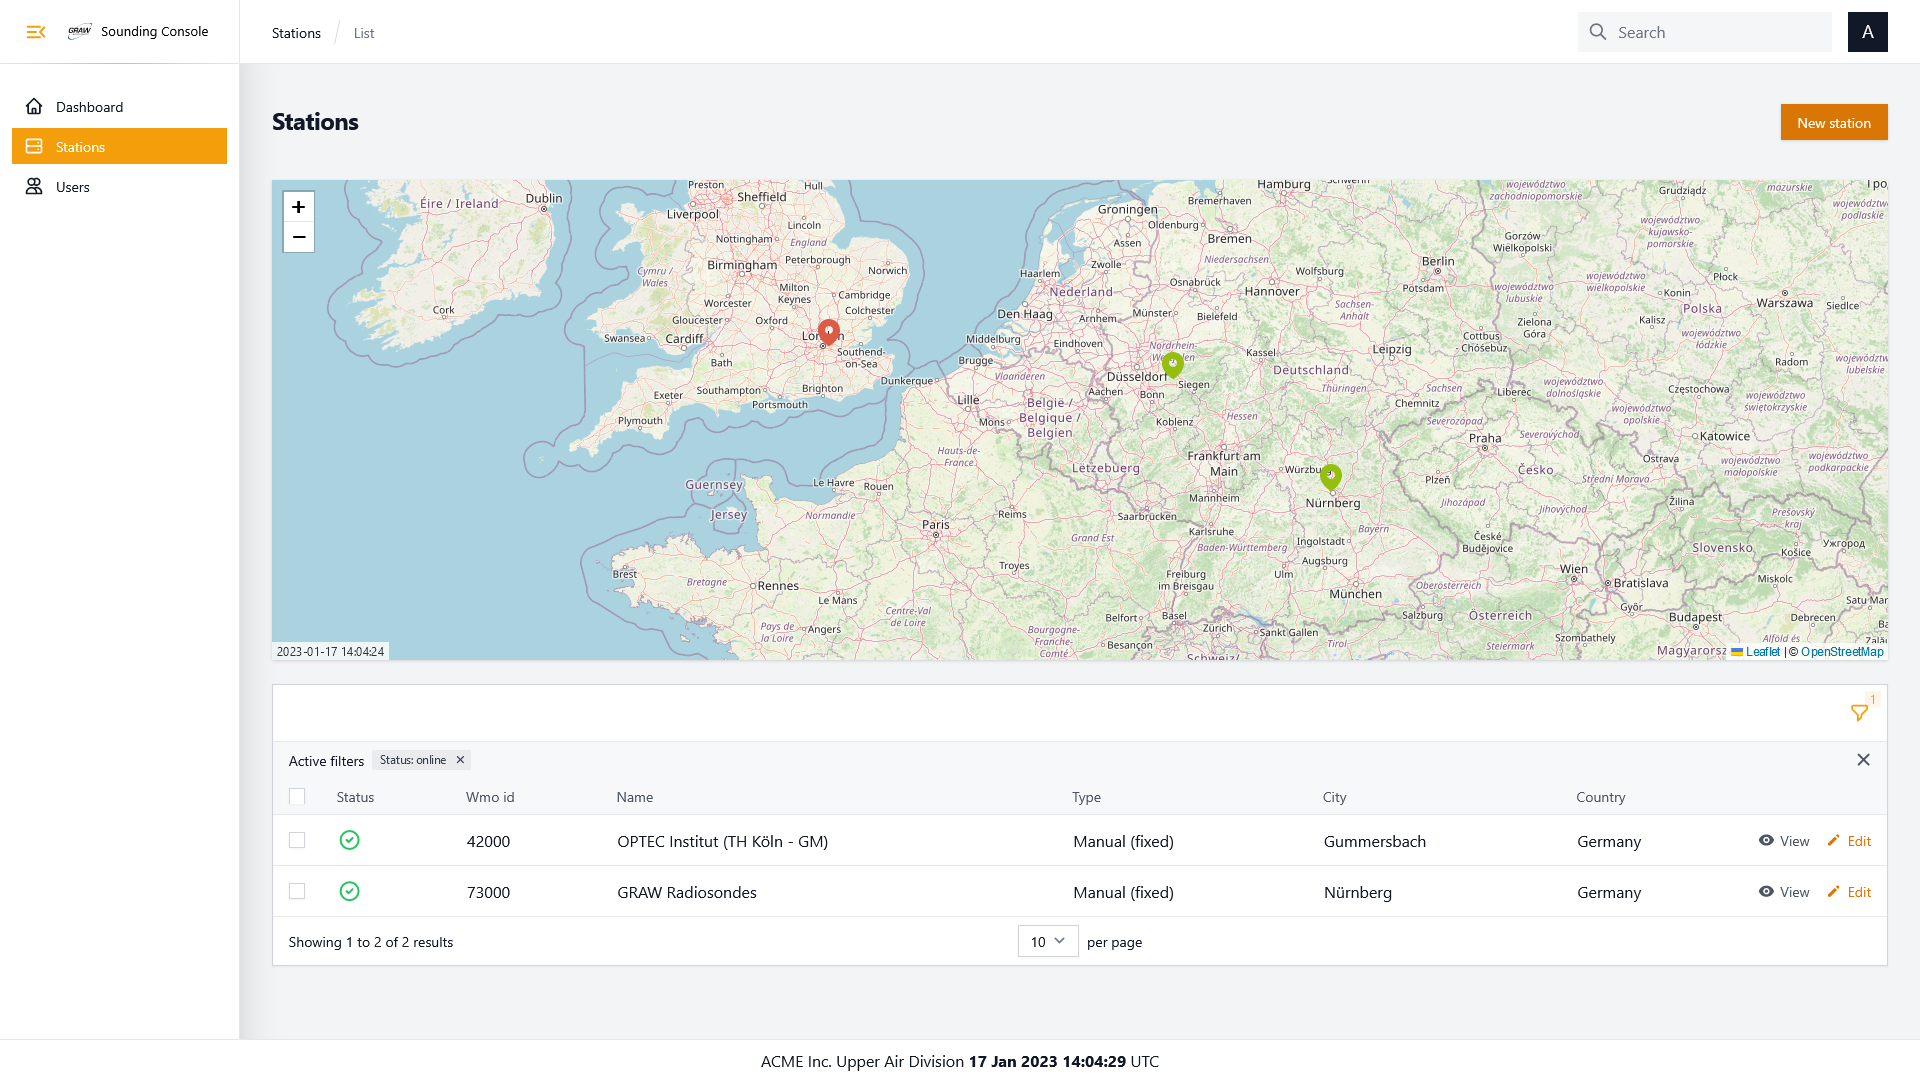
\includegraphics[scale=0.23]{assets/active_filter_filament}}
\end{figure}

\begin{figure}[h!]
    \centering
    \caption{Nova: aktiver Filter}
    \label{fig:active_filter_nova}
    \frame{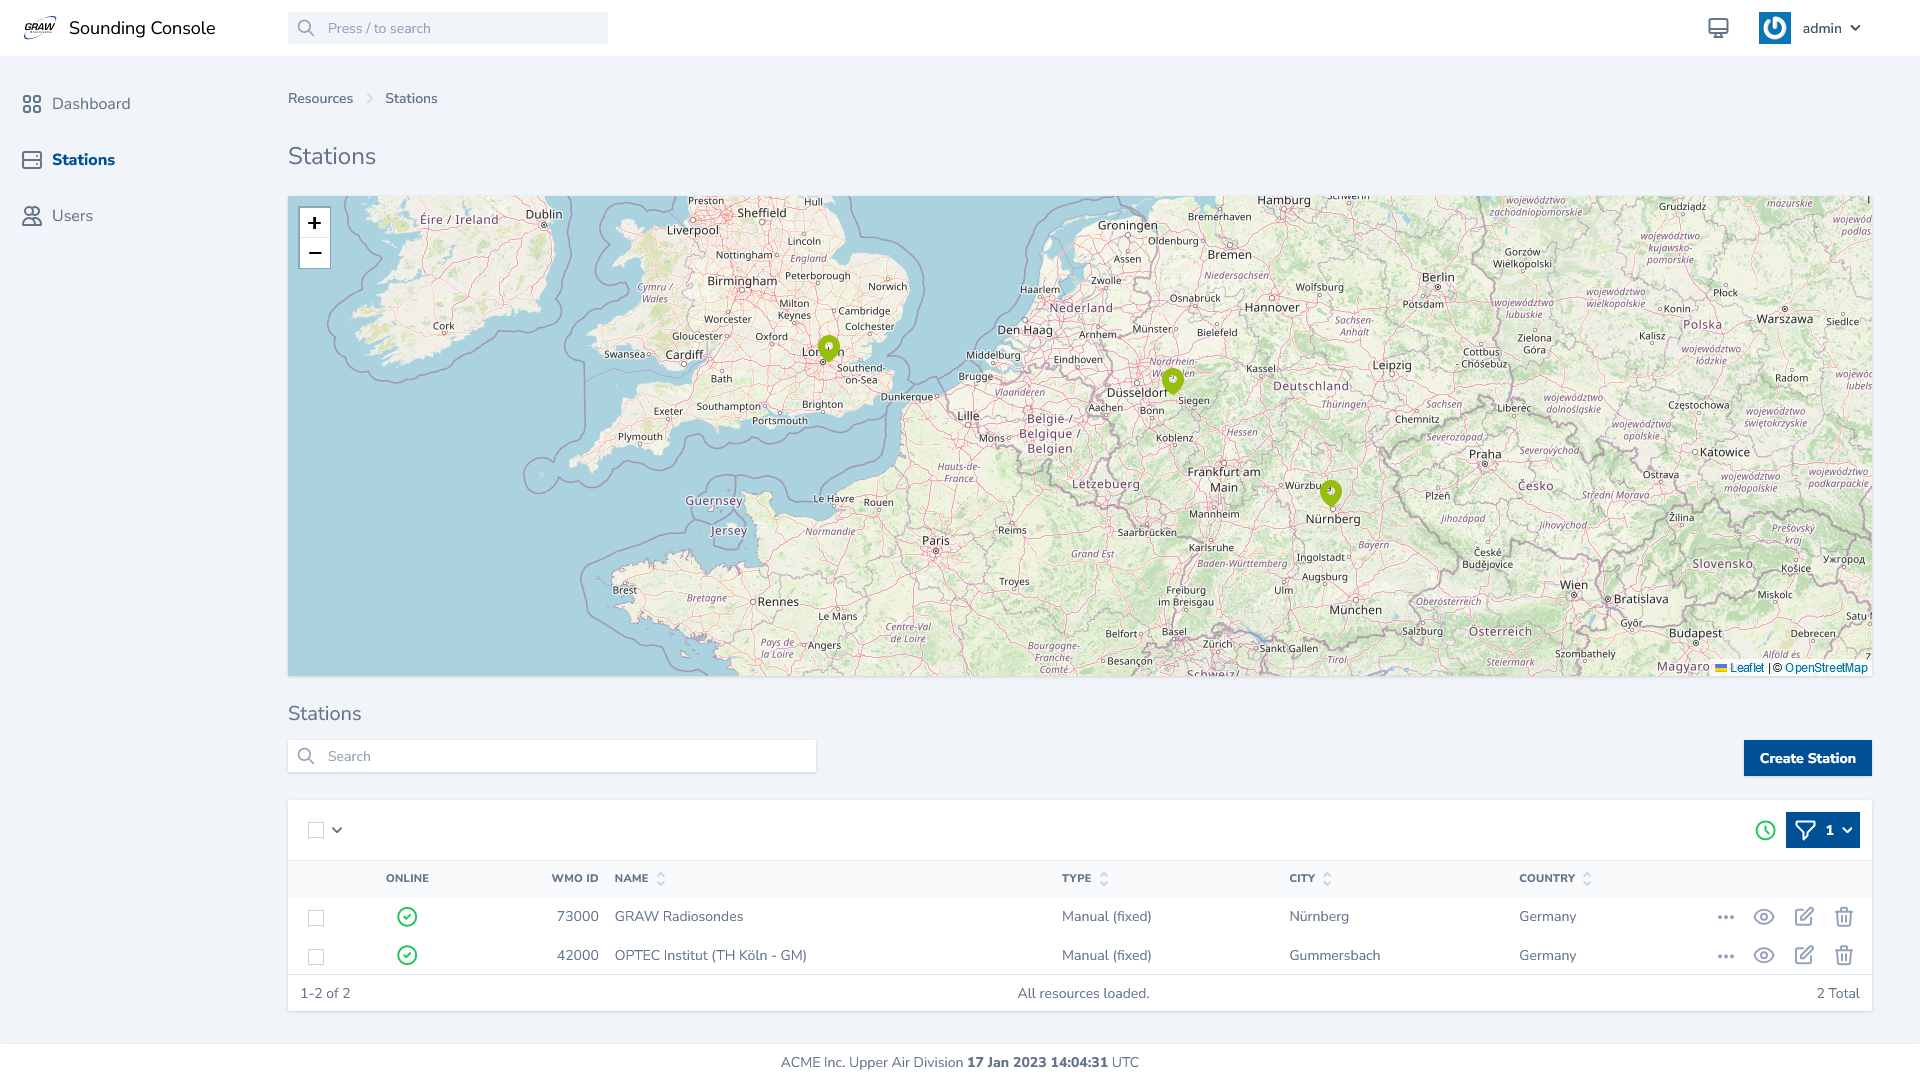
\includegraphics[scale=0.23]{assets/active_filter_nova}}
\end{figure}
\color{black}

\newpage

\newlineparagraph{Flight View Anpassbarkeit}
Manche Ansichten benötigen weitreichende Anpassungen.
Hierzu zählt speziell der Blick auf einen vergangenen Flug.
Bei laufenden Flügen wird lediglich ein Dashboard mit aktuellen Werten und eine Karte angezeigt.
Beides lässt sich sinnvoll oberhalb der restlichen Komponenten der Ressource, den Stammdatenfeldern und der Messwertetabelle, platzieren.

Im Fall von vergangenen Flügen fällt das Dashboard weg, jedoch kommen ein Messdatendiagramm, eine Statistikübersicht und ein Skew-T-Diagramm hinzu.
Insgesamt sind das zu viele und zu große Komponenten, um sie unmittelbar oberhalb auf der Seite zu platzieren.
Ein User müsste viel scrollen, um alles zu erfassen.
Dies wäre unübersichtlich und ineffizient.

Nova bietet kaum Möglichkeiten eine Ansicht anzupassen.
Daher war es die beste Variante, die Komponenten in Unterpunkte auszulagern (\ref{fig:finished_flight_nova}).
Nova unterstützt sogenannte Tools, welche eigenständige Seiten sind und auf denen individuelle Komponenten implementiert werden können.
Außerdem kann kontextabhängig das Menü angepasst werden.
Tests erster Nutzer zeigten jedoch, dass die entworfene Navigationsstruktur zu unübersichtlich ist.

\newpage

\begin{figure}[h!]
    \centering
    \caption{Nova: abgeschlossener Flug}
    \label{fig:finished_flight_nova}
    \frame{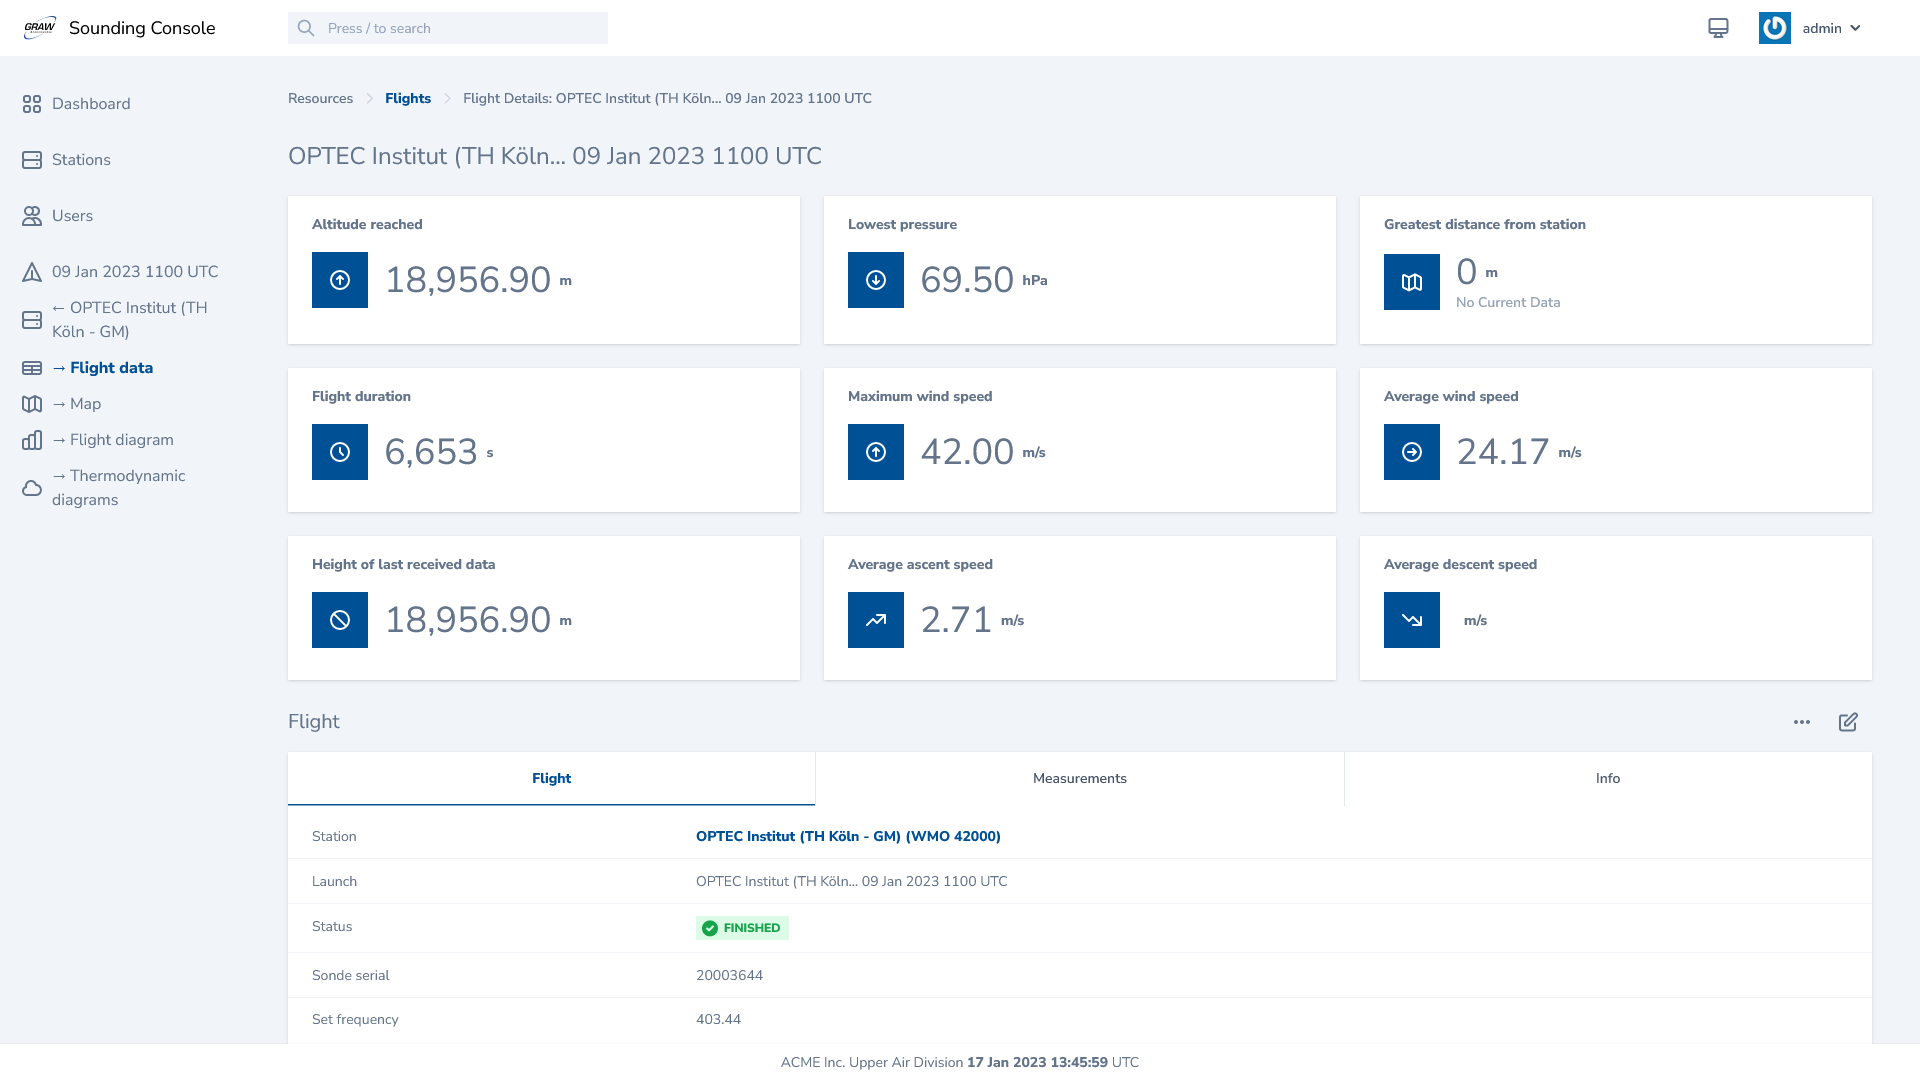
\includegraphics[scale=0.23]{assets/finished_flight_nova}}
\end{figure}

Filament bietet gegenüber Nova weitaus mehr Möglichkeiten, eine Ansicht individuell anzupassen.
So kann bei der vorliegenden Herausforderung eine individuelle View für den Header angegeben werden.
Diese wird oberhalb aller anderen Komponenten auf der Ansichtsseite eines Fluges gerendert.
Innerhalb dieser individuellen View kann dann eine Tab View implementiert werden, die immer nur eine größere Komponente auf einmal anzeigt (\ref{fig:finished_flight_filament}).

Die Lösung mit filament überzeugt durch eine deutlich bessere User Experience.
Die komplizierte Navigationsstruktur im Menü entfällt komplett und alles findet direkt innerhalb der Flugansicht statt.
Längeres Scrollen entfällt und die Ansicht bleibt kompakt und übersichtlich.
Insofern überzeugt filament an dieser Stelle durch die flexible und umfangreiche Anpassbarkeit.

\begin{figure}[h!]
    \centering
    \caption{Filament: abgeschlossener Flug}
    \label{fig:finished_flight_filament}
    \frame{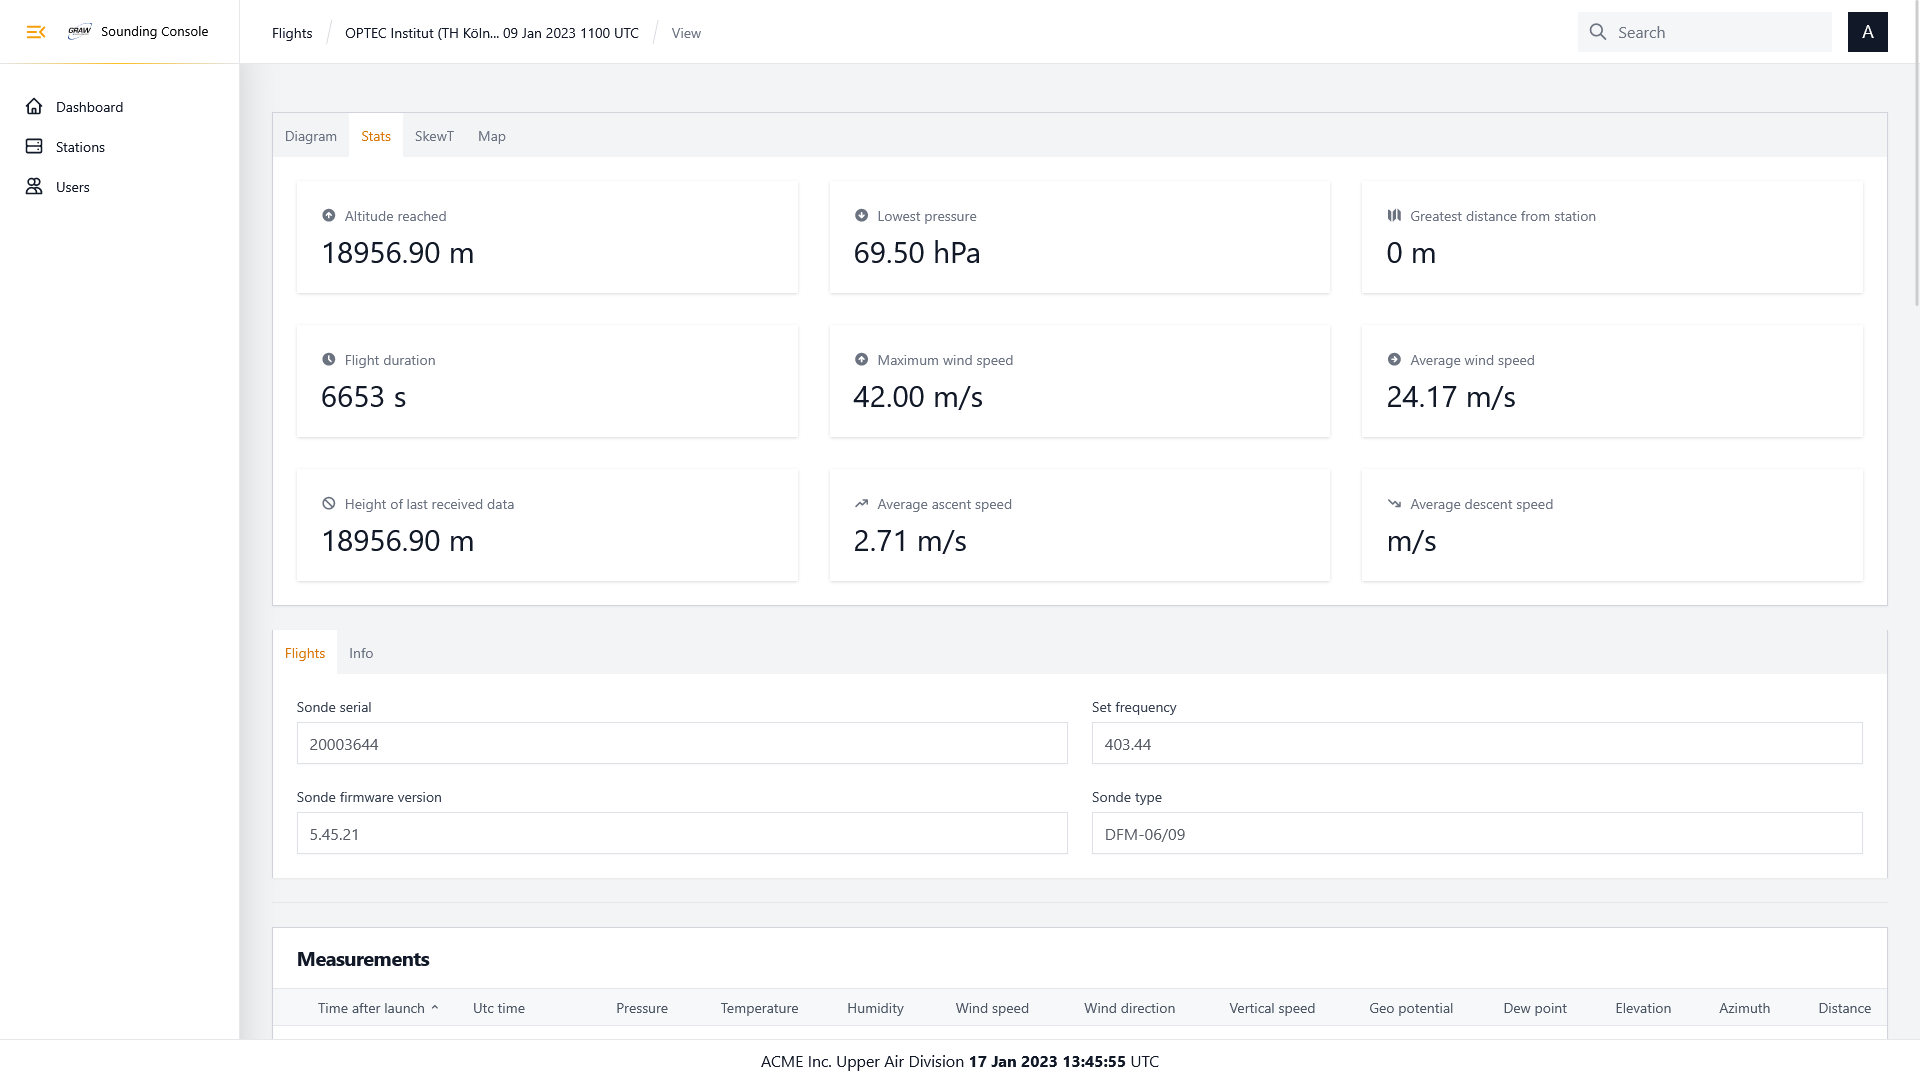
\includegraphics[scale=0.23]{assets/finished_flight_filament}}
\end{figure}

\newpage

\newlineparagraph{Generelle Anpassbarkeit}
Filament punktet insgesamt, durch eine flexiblere Anpassbarkeit, beispielsweise die Styles lassen sich besser modifizieren.
Des Weiteren gibt es die Möglichkeit, an vielen Stellen individuelle Views einzuhängen.

\newlineparagraph{Ladeanimation der aktualisierenden Tabelle}
Filament zeigt keine Ladeanimation an, wenn die Tabelle neue Daten pollt.
Dadurch ist ein einfacher Vergleich der Werte möglich und die Seite springt nicht, außer es kommen neue Einträge hinzu.
Insgesamt ist die User Experience durch diese Animation bei filament wesentlich besser als bei Nova.

\newlineparagraph{Livewire Polling (Flight Dashboard Component)}
Filament basiert auf Livewire\cite{livewire} und somit können innerhalb einer individuellen Komponente auch Funktionen von Livewire genutzt werden.
Beispielsweise gibt es einen eingebauten Polling Mechanismus.
Es muss lediglich ein Attribut zu einem HTML Objekt hinzugefügt werden und Livewire ruft dieses in einem definierbaren Intervall erneut vom Server ab.

Auf diese Weise wurde die Implementierung des Dashboards eines laufenden Fluges vereinfacht.
Die Api und das manuelle Polling mit anschließendem Austausch der Datenbasis, damit Vue.js den Inhalt dann reaktiv updaten kann, werden nicht mehr benötigt.
Es muss lediglich innerhalb der Blade Komponente mit serverseitigem Code das Dashboard generiert werden und Livewire übernimmt den Rest vollautomatisch.

\newpage

\newlineparagraph{Styling von Custom Components}
Nova unterstützt explizit die Verwendung der Blade Components.
So können fertige Funktionen und einheitliche Stile wiederverwendet werden.
Bei der Sounding Console werden beispielsweise Widgets als fertige Komponente geladen.

\newlineparagraph{Infinite Loading Tables}
Filament schafft es, eine benutzbare UI mit mehreren tausenden geladenen und angezeigten Zeilen in einer Tabelle zu rendern.
Damit ist im Gegensatz zu Nova kein Infinite Load/Scroll Pattern notwendig.

Außerdem zeigt filament standardmäßig auch eine \enquote{All} Option für die Pagination an.
Dadurch kann eine zu nativen Anwendungen vergleichbare UI erstellt werden, in welcher der User durch die vollständige Tabelle scrollen kann.

\newlineparagraph{Tabellensortierung}
Ist bei filament eine Spalte als sortierbar definiert, kann für eine Ansicht ebenfalls eine Standardsortierung angegeben werden.
Dabei ist sowohl die Angabe der Spalte möglich, als auch die Sortierrichtung.
Das Problem mit Nova wird, durch diese implementierte Lösung, vollständig gelöst.

\subsubsection{Negative Erfahrungen}
Trotz aller positiven Erfahrungen gab es auch eine Hürde mit filament, welche im Folgenden erläutert ist.
Diese konnte allerdings, mit der Umstellung auf ein neues Konzept, überwunden werden.

\newlineparagraph{Livewire Polling (Map Component)}
Das Livewire Polling Konzept ist nicht immer von Vorteil.
Bei einfachen Komponenten ist es sinnvoll, bei komplexeren Komponenten wie zum Beispiel der Karte, ist es problematisch.
Mit Nova war die Umsetzung etwas einfacher, da individuelle Nova Komponenten bereits eine geschützte HTTP Api vorbereiten, über die Updates regelmäßig abgerufen werden können.
Das Polling der gesamten Komponente ist mit filament keine Option, dennoch müssen Veränderungen erkannt und automatisch angezeigt werden.
Durch das Attribut \enquote{wire:ignore} können dabei einzelne Bestandteile ausgenommen werden.
So wird die Karte und das dazugehörige Script nicht erneut geladen, sondern nur ein Teil, welcher bei einem Update ein Event aussendet, auf welches die Karte dann reagiert.

\newpage

\subsubsection{Implizit versus explizit}
Die prototypischen Erfahrung entsprechen denen, über die andere Entwickler\cite{reddit-laravel-nova-vs-filament} bereits berichteten.
Nova arbeitet impliziter als filament:
Felder werden an einer Stelle definiert, diese gelten dann sowohl für das Formular, als auch für die Tabelle (\ref{fig:station_fields_nova}).
Bei filament wird ein Feld mindestens an zwei Stellen definiert (\ref{fig:station_fields_filament}).

\begin{figure}[h!]
    \centering
    \caption{Nova: Felddefinition Station}
    \label{fig:station_fields_nova}
    \frame{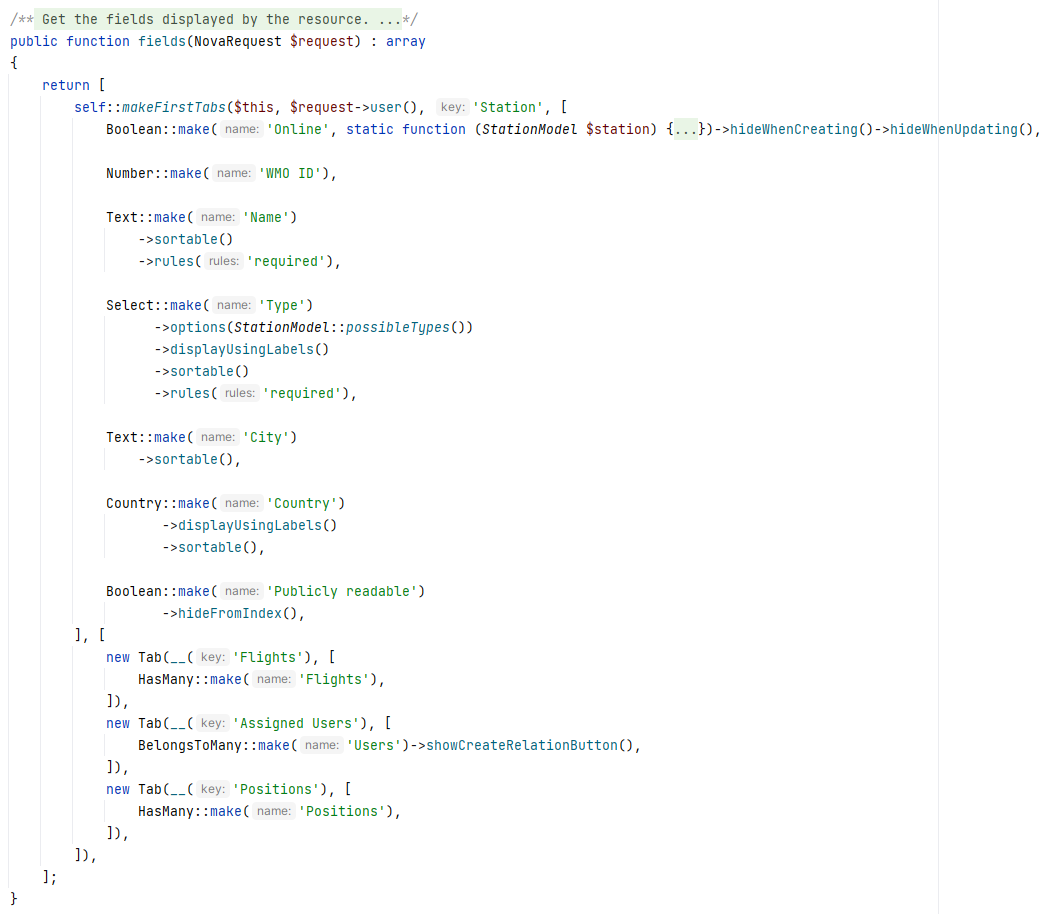
\includegraphics[scale=0.60]{assets/station_fields_nova}}
\end{figure}

Grundsätzlich erwartet filament, dass für jede eigene Tabelle die Spalten erneut explizit definiert werden.
Dies lässt sich jedoch umgehen, indem die Tabelle aus der Ressource referenziert wird.

Die unterschiedlichen Ansätze haben ihre Vor- und Nachteile.
Der implizite Ansatz bei Nova ist schneller, insbesondere am Anfang.
Filaments explizite Definitionen benötigen initial mehr Zeit, überzeugen aber am Ende durch eine bessere und einfachere Anpassbarkeit.
Zudem ist es durchaus sinnvoll explizit zu formulieren, wie die Felder im Formular und wie sie in Tabellen dargestellt werden sollen.
So wird verhindert, dass unerwartete Fälle eintreten, da die explizite Definition jedes Falls während der Entwicklung, mindestens einmal durchdacht werden muss.

\begin{figure}[h!]
    \centering
    \caption{Filament: Felddefinition Station}
    \label{fig:station_fields_filament}
    \frame{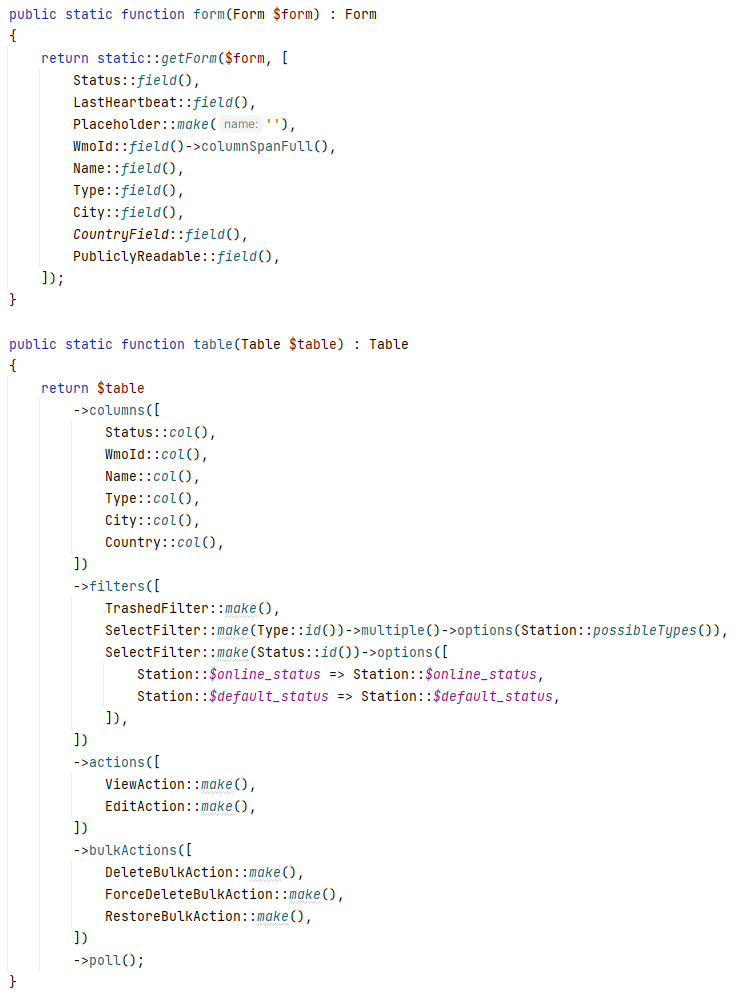
\includegraphics[scale=0.60]{assets/station_fields_filament}}
\end{figure}

\newpage
\subsection{Vergleich des Funktionsumfangs}
In nachfolgender Tabelle~\ref{tab:feature-comparison} sind alle verglichenen Features und die dazugehörigen Bewertungen gelistet.
Es ergibt für Nova einen Score von 10 und für filament einen Score von 34.
Damit ist der Vergleich der Features eindeutig und filament kann hier deutlich überzeugen.
Bei diesem hohen Punkteunterschied wäre selbst bei einer anderen Gewichtung der Aspekte der Features davon auszugehen, dass filament bei der quantitativ Betrachtung besser abschneiden würde.

Qualitativ überzeugt filament ebenfalls, da insbesondere im Bereich der Customization mehr Features und umfangreichere Optionen vorhanden sind.
Dies ist insofern relevant, da in der vorherigen Arbeit mit Nova vor allem die Anpassbarkeit ein Problem war.
Nova überzeugt gegenüber filament im Bereich Search.
Dieser Aspekt ist im Projekt Sounding Console allerdings nicht wesentlich.

Abschließend überzeugt filament sowohl quantitativ durch das Featureset als auch qualitativ aufgrund der wesentlichen und gut umgesetzten Features.

\begin{table}[h!]
    \label{tab:feature-comparison}
    \resizebox{\textwidth}{12.2cm}{%
        \begin{tabular}{llclcl}
            \textbf{Category}                        & \textbf{Feature}       & \textbf{10} & \textbf{Nova}                   & \textbf{34} & \textbf{Filament}                        \\
            \hline
            \multirow{2}{*}{\textbf{Technical}}      & Laravel Support        & n           & \textgreater{}= 8.0             & n           & \textgreater{}= 8.0                      \\
            & PHP Support            & g           & \textgreater{}= 7.3             & n           & \textgreater{}= 8.0                      \\
            \hline
            \multirow{10}{*}{\textbf{Resources}}     & Number of fields       & g           & 38                              & b           & 16                                       \\
            & Computed fields        & g           & yes                             & g           & yes                                      \\
            & Repeater fields        & b           & no                              & g           & supported                                \\
            & Builder fields         & b           & no                              & g           & supported                                \\
            & Table polling          & n           & yes, but bad animation          & g           & yes                                      \\
            & Filters                & g           & supported                       & g           & supported                                \\
            & Lenses                 & g           & supported                       & b           & no                                       \\
            & Actions                & n           & title, fields \& responses      & g           & title, fields, responses \& custom views \\
            & Queued Actions         & g           & supported                       & n           & only custom                              \\
            & Action log             & g           & supported                       & b           & no                                       \\
            \hline
            \multirow{3}{*}{\textbf{Custom views}}   & Custom pages/Tools     & n           & complicated but powerful        & g           & simple and powerful                      \\
            & Custom resource pages  & b           & no                              & g           & yes                                      \\
            & Widgets/Cards          & n           & complicated but powerful        & g           & simple and powerful                      \\
            \hline
            \multirow{12}{*}{\textbf{Search}}        & Searchable Columns     & g           & can be defined                  & g           & can be defined                           \\
            & Title                  & g           & can be defined                  & g           & can be defined                           \\
            & Details/Subtitle       & g           & can be defined                  & g           & can be defined                           \\
            & Url                    & b           & no                              & g           & can be defined                           \\
            & Actions                & b           & no                              & g           & can be defined                           \\
            & Full-Text Indexes      & g           & supported                       & b           & no                                       \\
            & Searching Relations    & g           & supported                       & b           & not clear, probably not supported        \\
            & Searching JSON Data    & g           & supported                       & b           & not clear, probably not supported        \\
            & Limits                 & g           & supported                       & b           & no                                       \\
            & Debounce timing        & g           & supported                       & b           & no                                       \\
            & Global disable         & g           & supported                       & b           & no                                       \\
            & Laravel Scout          & g           & supported                       & n           & can be customized                        \\
            \hline
            \multirow{15}{*}{\textbf{Metrics}}       & Value                  & g           & avg/sum/max/min                 & n           & yes, but no predefined functions         \\
            & Trend/Line             & g           & count/avg/sum/max/min           & n           & yes, but no predefined functions         \\
            & Bar                    & b           & no                              & g           & yes                                      \\
            & Bubble                 & b           & no                              & g           & yes                                      \\
            & Polar Area             & b           & no                              & g           & yes                                      \\
            & Radar                  & b           & no                              & g           & yes                                      \\
            & Scatter                & b           & no                              & g           & yes                                      \\
            & Partition/Pie/Doughnut & g           & avg/sum/max/min                 & n           & yes, but no predefined functions         \\
            & Progress               & g           & count/sum                       & b           & no                                       \\
            & Custom chart control   & b           & no                              & g           & yes, configure the chart.js options      \\
            & Table                  & n           & icon, title, subtitle \& action & g           & multiple columns, filters \& actions     \\
            & Ranges                 & g           & can be defined                  & g           & can be defined                           \\
            & Caching                & g           & supported                       & b           & no                                       \\
            & Formatting             & n           & possible but limited            & g           & possible                                 \\
            & Polling                & n           & some events                     & g           & interval                                 \\
            \hline
            \multirow{3}{*}{\textbf{Dashboard}}      & widget width           & n           & yes                             & g           & yes, responsive                          \\
            & grid col number        & b           & no                              & g           & yes, responsive                          \\
            & conditionally hiding   & g           & yes                             & g           & yes                                      \\
            \hline
            \multirow{5}{*}{\textbf{Notifications}}  & Content                & n           & title, action, icon \& type     & g           & title, body, action, icon \& type        \\
            & Global disable         & g           & supported                       & b           & no                                       \\
            & Duration               & b           & no                              & g           & supported                                \\
            & Persistent             & b           & no                              & g           & supported                                \\
            & Custom view            & b           & no                              & g           & supported                                \\
            \hline
            \multirow{2}{*}{\textbf{Navigation}}     & Customize Main Menu    & g           & yes                             & g           & yes                                      \\
            & Customize User Menu    & g           & yes                             & g           & yes                                      \\
            \hline
            \multirow{10}{*}{\textbf{Customization}} & Logo                   & n           & only SVG file                   & g           & custom view                              \\
            & Dark Mode              & n           & switch can be disabled          & g           & mode and switch can be enabled           \\
            & Collapsible sidebar    & b           & no                              & g           & yes                                      \\
            & Themes                 & n           & colors can be changed           & g           & full theme can be extended               \\
            & Max content width      & b           & no                              & g           & changeable globally or per page          \\
            & Custom Assets          & n           & only by overwriting the layout  & g           & hooks to register styles/scripts         \\
            & Meta tags              & n           & only by overwriting the layout  & g           & yes, via hook                            \\
            & Notification position  & b           & no                              & g           & vertical and horizontal alignment        \\
            & Render hooks           & b           & no                              & g           & add custom views in 28 places            \\
            & Footer                 & n           & only text                       & g           & custom view                              \\
            \hline
            \multirow{3}{*}{\textbf{Plugins}}        & Total                  & n           & 816                             & n           & 158                                      \\
            & Current                & g           & 161                             & g           & 158                                      \\
            & Repository             & n           & third-party\cite{nova-packages} & g           & first-party\cite{filament-plugins}       \\
            \hline
            \multirow{3}{*}{\textbf{Other}}          & Impersonation          & g           & yes                             & b           & no                                       \\
            & Localization           & g           & yes                             & g           & yes                                      \\
            & Modal resources        & b           & no                              & g           & yes
        \end{tabular}%
    }
    \caption{Featurevergleich}
\end{table}


\newpage
\subsection{Maturity im Vergleich}
Unter Anwendung des TRL (Technology Readiness Level) ließen sich keine Unterschiede zwischen Nova und filament feststellen.
Im Rahmen dieser Arbeit würden beide Umsetzungen Level 7 erreichen, da eine prototypische Demo in einer operativen Umgebung fertiggestellt ist.
Werden jedoch die Berichte aus der Community als Basis zugrunde gelegt, so müssen beide Frameworks auf Level 9, dem höchsten Level, eingeordnet werden.
Sowohl für Nova als auch für filament laufen erfolgreiche Anwendungen im Produktivbetrieb.
(Vgl.~\cite{technology-readiness})

Eine stabile Version von Nova wurde erstmals am 22.08.2018\cite{nova-releases} veröffentlicht und ist damit etwa viereinhalb Jahre alt.
Filament ist wesentlich jünger.
Das erste stable Release erfolgte am 02.03.2021\cite{filament-releases}, also vor knapp zwei Jahren.

Nova ist folglich mehr als doppelt so lange verfügbar wie filament und befindet sich inzwischen in der vierten Hauptversion\cite{nova-releases}.
Filament hat bisher die zweite Hauptversion\cite{filament-releases} erreicht.
Wird das Alter der Technologie als Indikator für die Reife herangezogen, so spricht dieses für Nova.

\subsubsection{Dokumentation}
Bei der praktischen Arbeit mit beiden Frameworks ist aufgefallen, dass die Dokumentation in beiden Fällen hervorragend ist.
Es war nie notwendig das Framework selbstständig nachzuvollziehen.
Alle relevanten Features sind ausführlich und an Beispielen beschrieben.
Auf Basis der Dokumentation lässt sich daher kein Favorit ermitteln, beide Frameworks schneiden gleich gut ab.

\subsubsection{Nutzerzahl}
Bei filament lassen sich konkrete Zahlen ermitteln (Stand: 08.01.2023 11:30 Uhr).
Packagist verzeichnet insgesamt 470.626 Installationen.
Bei GitHub gibt es 5.4k Stars, 795 Forks und 91 Watcher.

Bei Nova hingegen lassen sich keine konkreten Zahlen ermitteln.
Es gibt lediglich ein offenes GitHub Projekt in dem Fehler gesammelt werden.
Dieses hat 525 Stars, 36 Forks und 58 Watcher.
Da diese Zahlen nicht vergleichbar sind, ist auf Basis der Nutzerzahlen keine Aussage möglich.

\subsubsection{Bekannte Fehler}
Nova listet aktuell 12 offene Issues, bei filament sind es 18, davon 7 für die kommende Version.
Der quantitative Blick auf die Fehlerdokumentationen lässt daher keinen Unterschied feststellen.

\subsubsection{Moderne Sprachfeatures}
Beide Frameworks laufen unter PHP 8.2 und damit unter der aktuell neusten Version.
Moderne Sprachfeatures können daher bei beiden Frameworks verwendet werden, hier ist kein Unterschied zu erkennen.

\subsubsection{Roadmap}
Bei Nova gibt es keine öffentliche Roadmap, entsprechend ist hier kein Vergleich möglich.

Bei filament ist seit mehreren Monaten die nächste Hauptversion (v3) in Entwicklung\cite{filament-v3-plans} und die Pläne werden offen kommuniziert.
Das Framework soll mit der nächsten Version nicht mehr nur für Admin Panels, sondern für jegliche Anwendung konzipiert werden\cite{filament-v3}.
Dies ist für das vorliegende Projekt der Sounding Console sehr interessant, da es hier bereits über ein Admin Panel hinaus verwendet wird.

Filament überzeugt basierend auf der Roadmap gegenüber Nova.
Die geplanten Features sind für den aktuellen Projektkontext sehr interessant.
Dazu gehören insbesondere der Support genereller Anwendungen, verbesserte Performance, visuell ansprechendere Views und zusätzliche Icons.

\subsubsection{Fazit Maturity}
Nova überzeugt durch ein wesentlich höheres Alter, filament durch die verfügbare Roadmap.
An dieser Stelle lässt sich hinsichtlich der Maturity kein Unterschied zwischen den beiden Frameworks feststellen.

\newpage
\subsection{Vergleich des Code Style}
\newlineparagraph{PSR}
Nova und filament basieren auf dem Framework Laravel.
Laravel folgt laut eigenen Angaben beim Autoloading der aktuellen PSR-4, beim Coding Style allerdings der veralteten PSR-2~\cite{laravel-docs-coding-style}.
Weder Nova noch filament erwähnen einen Code Style in der jeweiligen Dokumentation.

Filament scheint Laravel Pint~\cite{laravel-docs-pint} zu verwenden, zumindest existiert im Projektrepository eine pint.json Datei mit der notwendigen Konfiguration.
Darin wird als Vorlage der Stil von Laravel verwendet und leicht angepasst.
An dieser Stelle wäre auch die PSR-12 möglich, filament scheint sich aber eher an dem Framework zu orientieren, auf dem es aufbaut.

Bei Nova findet sich im Projektverzeichnis ebenfalls eine pint.json Datei mit der Laravel Vorlage.
Dies ist auch erwartbar, da es sich bei Nova um ein first-party Package handelt.

Zusammenfassend lässt sich also sagen, dass beide Frameworks sich nicht direkt an die aktuelle PSR halten, sondern an die Vorgaben von Laravel selbst.
Die Laravel Standards basieren jedoch zumindest teilweise auf den PSR Standards.

\newlineparagraph{Clean Code}
Die Heuristiken für sauberen Code nach Robert C. Martin sind sehr umfangreich, insgesamt 63, ausgenommen der Java spezifischen.
Im Folgenden wird daher nur ein grober und zusammenfassender Blick auf die Anwendung dieser Heuristiken in den beiden Frameworks geworfen.

Grundsätzlich lässt sich feststellen, dass beide Frameworks sich an die Regeln für Kommentare halten.
Die Umgebung ist ebenfalls einfach einzurichten und erfordert keine komplizierten Schritte, um lauffähig zu werden.
Funktionsargumente sind meist eher wenige und es wird meist sauber mit veränderlichen Objekten gearbeitet.

Die Absicht des Frameworkcodes ist in der Regel klar und deutlich.
Benennungen von Variablen und Funktionen sind beschreibend, eindeutig und enthalten keine unnötigen Präfixe.
Bezüglich der Testabdeckung lässt sich bei beiden Frameworks keine Aussage treffen.

Grundsätzlich lässt sich bei beiden Frameworks kein wirklicher Unterschied bezüglich der \enquote{Sauberkeit} des Codes feststellen.

\newpage

\newlineparagraph{Typisierung}
Bei den zu erweiternden Klassen fallen Unterschiede zwischen den Frameworks auf.
Nova typisiert den Code nur in Teilen.
Vor allem Funktionsparameter sind typisiert, Rückgabewerte nicht immer und Klassenattribute meistens nicht.
Bei filament stellt sich dies anders dar.
In der betrachteten Stichprobe waren die Klassen vollständig typisiert.
Die Qualität des filament Codes ist in diesem Aspekt daher wesentlich höher.

\newpage
\subsection{Kostenvergleich/Lizenzierung}
Die Kosten beim Einsatz von Nova und filament unterscheiden sich deutlich.
Filament ist eine quelloffene Entwicklung unter der MIT-Lizenz.
Dadurch sind die vollständige Nutzung, Veränderungen und der Vertrieb möglich.
Es entstehen keine Kosten und eine Weiterentwicklung wäre auch durch neue Entwickler möglich, sollten die aktuellen Entwickler das Projekt einstellen.

Nova hingegen kostet für unlimitierte Projekte einmalig 299 Dollar.
Durch die On-Premise Bereitstellung ist diese größere Lizenz notwendig.
Diese Lizenz ermöglicht Updates für ein Jahr, danach fallen erneut Kosten an.
Da Updates notwendig sind, ist mit jährlich wiederkehrenden Kosten zu rechnen.
Gleichwohl fallen bei beiden Frameworks Personalkosten an.
Mit Blick hierauf sind die Lizenzkosten vergleichsweise niedrig.

Bei der Betrachtung der Lizenzkosten schneidet filament somit besser ab.
Neben den fehlenden Lizenzkosten ist vor allem die quelloffene Entwicklung von Vorteil, insbesondere hinsichtlich langer Produktlebenszyklen.

\newpage
\subsection{Rückmeldungen aus der Community}
Im Laravel Subreddit wurde die Frage gestellt, ob Nova oder filament für ein mittelgroßes Admin Panel geeigneter ist\cite{reddit-laravel-nova-vs-filament}.
Dort finden sich die folgenden Antworten auf diese Frage:

\begin{itemize}
    \item \enquote{I have worked with both and found Filament much easier to work with.}
    \item \enquote{Another problem I encountered with Nova is that customers without a technical background have a difficult time to work with Nova.}
    \item \enquote{Customising nova is really difficult.}
    \item \enquote{I've used both, and i still use both, but i prefer filament for it's community and easy customization, but i still use nova for vue projects.}
    \item \enquote{Nova is perfect if you don't need customization}
    \item \enquote{In my experience if you don’t need alot of custom work use Nova cause it’s easier and way faster to develop with.}
    \item \enquote{If you need something custom use filament.}
    \item \enquote{Filament is a lot easier to customize and extend. Mainly because you don’t have the compile Vue, etc.}
\end{itemize}

Insgesamt wird filament als anpassbarer und einfacher in der Handhabung beschrieben.
Durch den TALL Stack (Tailwind, Alpine.js, Laravel \& Livewire) fällt Vue.js im Frontend weg und damit die Notwendigkeit den Code zu kompilieren.
Nova wird bevorzugt, wenn keine Anpassungen benötigt werden, da es als einfaches Admin Panel schneller konfiguriert ist.


    \addtocontents{toc}{\protect\newpage}

\newpage


\section{Ergebnisse und Reflektion}

\subsection{Ergebnisse}
\color{red}
tbd
\color{black}

\subsection{Kritischer Rückblick}
\color{red}
tbd
\color{black}

    \newpage

\section{Fazit und Ausblick}

\subsection{Fazit}
\color{red}
tbd
\color{black}

\subsection{Ausblick}
Aufgrund des eindeutigen Fazits zugunsten des Einsatzes von filament soll die Sounding Console zeitnah vollständig auf filament umgestellt werden.
Dafür müssen die wenigen, gegenüber dem MVC mit Nova fehlenden, Features implementiert werden.

Im Anschluss daran soll eine erste interne Testphase starten und die Software von mehreren Nutzern evaluiert werden.
Danach soll die Software bei den ersten Messnetzwerken in Betrieb gehen.

Bisher wurden realistische Lasttests noch nicht durchgeführt.
Diese wurden bereits im Ausblick der Praxisprojektarbeit angekündigt und die Bearbeitung ist bereits gestartet.
Jedoch wurde zunächst der Vergleich mit, sowie der Umbau auf filament priorisiert.
Da bei den Lasttests kein Browser ausgeführt wird, sondern nur HTTP Endpunkte abgerufen werden, ist das Testing von filament voraussichtlich besser zu bewerkstelligen.
Nova setzt viel auf Code im Frontend und führt auch dort das Routing durch.
Filament setzt die meisten Funktionen rein im Backend um und lässt sich insofern mit der angestrebten Testmethode auch besser testen, als dies bei Nova der Fall wäre.

Sobald die Software sich auch im produktiven Betrieb bewiesen hat, sollen weitere Funktionen, zum Beispiel für automatisierte Bodenstationen, sogenannte Autolauncher, implementiert werden.
Hierzu liegen derzeit jedoch nur grobe Pläne vor.


    \appendix

\newpage


\section{Quellenverzeichnis}
\bibliographystyle{plain}
\printbibliography


\section{Abbildungsverzeichnis}
\listoffigures

\newpage


\section{Anhang}

\subsection{Eigenständigkeitserklärung}

\textbf{Eidesstattliche Erklärung}

Ich versichere, die von mir vorgelegte Arbeit selbständig verfasst zu haben.

Alle Stellen, die wörtlich oder sinngemäß aus veröffentlichten oder nicht veröffentlichten Arbeiten anderer entnommen sind, habe ich als entnommen kenntlich gemacht.
Sämtliche Quellen und Hilfsmittel, die ich für die Arbeit benutzt habe, sind angegeben.

Die Arbeit hat mit gleichem Inhalt bzw.\ in wesentlichen Teilen noch keiner anderen Prüfungsbehörde vorgelegen.


\includegraphics[scale=0.5]{assets/signature}\\
Gummersbach, den \today

\end{document}
